\documentclass{article}
\usepackage{graphicx} % Required for inserting images
\graphicspath{ {./images/} }
\usepackage{dsfont}

\usepackage{listings}
\usepackage{xcolor}

\lstset{
    language=Python,
    basicstyle=\ttfamily\small,
    commentstyle=\color{green!50!black},
    keywordstyle=\color{blue},
    stringstyle=\color{orange},
    showstringspaces=false,
    numbers=left,
    numberstyle=\tiny\color{gray},
    numbersep=5pt,
    breaklines=true,
    breakatwhitespace=true,
}


\begin{document}

\begin{titlepage}
   \begin{center}
       \vspace*{1cm}

       \textbf{How Airlines  Fair (Fare)}

       \vspace{0.5cm}
An Analysis of how Ticket Prices Impact Value by Airline            
       \vspace{1.5cm}

       \textbf{Shivam Kak, Edward Zhang, Michael Perry, Pieter Heesters}

       \vfill
            
       An investigative study for the 2023 Citadel Invitational Datathon
            
       \vspace{0.8cm}
     
            
       Citadel, LLC.\\
       Miami, Florida\\
       USA\\
       30 July 2023
            
   \end{center}
\end{titlepage}


\begin{abstract}
    \textit{Despite having faced numerous economic events in the past decades, the airline industry continues to play a key role in the US economy. For this reason, gaining insights on a resilient industry can be invaluable moving forward. In this paper, we investigate numerous factors surrounding the value of a flight's fare, including the differing value from airline to airline, impact on delays, and prediction of delay time. First, we illustrate how some airlines offer better value due to a lower average fare per mile. Second, we investigate a positive correlation between fare price and delay time, suggesting that cheaper flights are less likely to be delayed. Finally, we created an XGBoost model to predict delay time due to airlines and output a probability distribution for possible delay times based on the airline, distance of trip, and average fare. Using our conclusions, flyers can be more informed when purchasing tickets as well as anticipate and plan for likely delays. }
\end{abstract}
\section{Introduction}
In today's highly interconnected world, the airline industry plays a pivotal role in facilitating global connectivity and economic growth. As our world becomes increasingly intertwined, understanding the dynamics of the airline industry and its impact on our economy is of utmost importance. In this datathon, we set out to explore the US airline industry, focusing on fare prices and their potential correlation with flight delays.


The US airline industry has been a vital engine of economic activity, demonstrating its resilience through numerous economic upheavals. Despite facing challenges, it has remained a critical driver in maintaining our physical connectivity and facilitating travel across the nation. We delved into pre-cleaned datasets encompassing various aspects of the airline industry in 2017, including airlines, airports, airline fares, and flight traffic. By using these datasets, we formed guiding research questions and then delved into the data. 

\subsection{Research Question}
In flights of equivalent distances, does the cost of airfare correlate to the probability of delays due to human error (factors other than weather)? A possible correlation may serve to raise ethical questions in the airline industry over why more expensive flights, which serve to drive more profits for airlines, are delayed less frequently. Building off of this question, this paper investigates how certain airlines may offer more valuable tickets per mile price. In addition, can a predictive model be generated to determine delay times due to human error, given an input of distance travelled, airline, and ticket price?

\subsection{Hypothesis}

Less expensive airfare tickets are likely to experience heightened delays due to human error, which includes air system delays, security delays, and airport delays. This correlation suggests that airlines may have a vested interest in prioritizing more expensive flights when it comes to resource allocation and minimizing delay times for customers deemed more valuable. This paper serves to analyze this pressing societal issue via the foreground of thorough data analysis. 



By exploring these questions, we can reach meaningful conclusions that keep flyers informed about the value of their ticket price and possibly improve their spending patterns. In our investigation, we can enlighten flyers on which airlines offer better pricing in terms of dollar per mile, as well as whether they can expect more or less delays depending on their ticket price. These insights are invaluable as flying is already an expensive endeavor and flyers want to spend their money smartly. 

Our primary objective in this datathon was to investigate whether there is a relationship between flight delays and fare prices. We aimed to understand if airlines tend to prioritize the punctuality of cheaper flights over those with higher average fares. Additionally, we endeavored to build a predictive model to estimate the delay time of a flight based on factors such as the airline, flight distance, and fare.

Through our thorough analysis, we discovered intriguing insights about the interplay between fare prices and flight delays. We found compelling evidence suggesting that the relationship between fare prices and delays is more complex than anticipated. Contrary to conventional belief, our findings indicate that fare prices alone  do not significantly impact flight delays. Instead, various other factors, such as airline operations, and air traffic, play crucial roles in determining delays.

To aid in future decision-making and enhance operational efficiency, we successfully developed a robust predictive model to estimate flight delay times. Our model's accuracy was impressive, demonstrating its potential to support airlines in better managing delays and improving passenger experiences.

In conclusion, our investigation into the US airline industry has shed light on the intricate dynamics of flight delays and fare prices. We hope that our findings and predictive model contribute to a deeper understanding of the airline industry's complexities and pave the way for more informed decision-making in this critical sector. As our world continues to evolve, a comprehensive understanding of the airline industry remains vital to sustain global connectivity and economic prosperity.

\section{Technical Summary}

Our main research topic was about getting the best value for your money from an airplane ticket. 

In the data preprocessing phase, we cleaned, transformed, and prepared the raw dataset to ensure its suitability for analysis. We addressed missing values, removed duplicates, standardized data formats, and merged datasets. 

Our first objective was to investigate the varying value of fares with respect to dollar per mile. By normalizing the ticket prices, this allowed us to fairly compare airlines' ticket costs. This investigation was done with rudimentary statistical operations on the fares dataset and then visualized with a bar graph. 

Our second objective was to investigate a possible correlation between fares and delays. After combining the dataset on fares and the dataset on flight traffic, we created groupings for flights based on airline and distance. After creating groups of roughly similar flights, we split each group into a cheap side and an expensive side based on the mean fare of the group, then compared the proportion of significantly delayed flights. For each group, we counted the proportion of times where the cheaper side was significantly delayed more and the proportion of times where the more expensive side was significantly delayed more; then, we represented these counts as a pie chart. In doing so, we found a relatively unexpected disparity: expensive flights are more frequently delayed. This finding was the basis for our third objective.

Our third objective was to create a model to predict delay times based on airline, trip distance, and flight fare. We first normalized using Min-Max normalization our features to ensure proper weighting and then fit these to an XGBoost model. This model allows us to predict a distribution of delays for a flight given airline, distance, and fare. 

Ultimately, we wanted to make airline delays less random to the average flyer and offer insights on probable indicators as well as illustrate the likeliness of different delays. While our model will likely fall short due to the minimal features, the model offers an accurate way to predict delays due to airlines.


\section{Ticket Price per Mile}
Our first investigation covers the varying value of fares purely with respect to distance: average fare per mile by airline. We used data from the US Department of Transportation in 2017 which had data on flights including their distance and numerous passenger ticket price buckets. Assuming the ticket prices within these bucket intervals are randomly distributed, we calculated the average fare for an airline as follows:
$$\textbf{Average Fare} = \frac{\sum (\textbf{Fare Bucket} \cdot \textbf{Passengers})}{\sum \textbf{Passengers}} $$
$$\textbf{Average Fare per Mile} = \frac{\textbf{Average Fare}}{\textbf{Distance}} $$
$$ \textbf{Average Fare per Mile}_{Airline X} = \frac{\sum (\mathds{1}\{Airline=X\} \cdot \textbf{Average Fare per Mile})}{\sum  \mathds{1}\{Airline=X\}} $$

With the corresponding average fare per mile for each airline, we created a bar graph to visualize the results, see the distribution, and understand which airlines offer the best value. 


\begin{center}
    \textbf{Figure 1}: Average Ticket Price per Mile by Airline
\end{center}
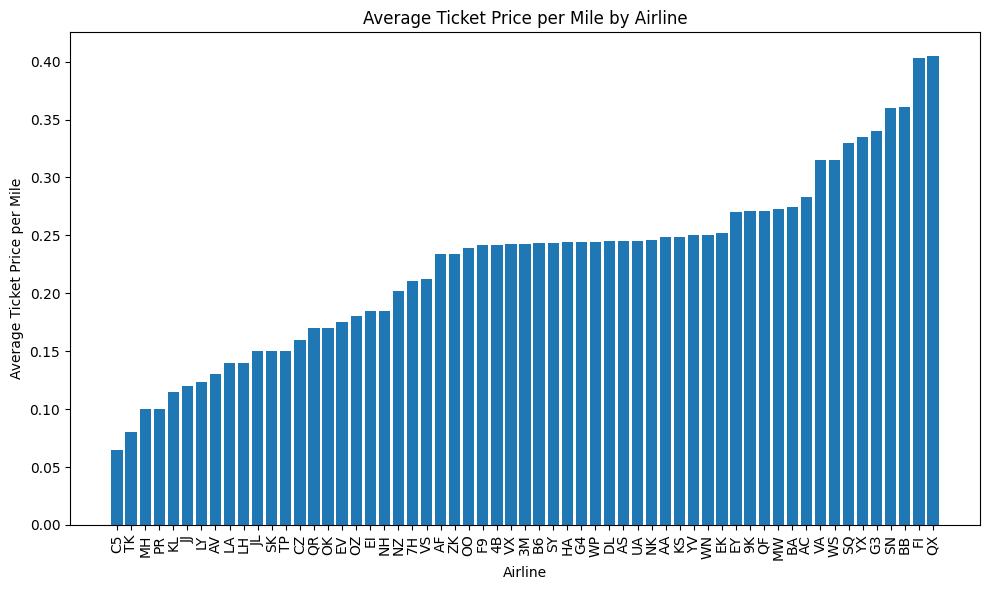
\includegraphics[scale=0.5]{images/AvgTicketPricePerMile.png}

As illustrated in Figure 1, there are clear disparities in the average price per mile with the biggest being Horizon Air Industries Inc. at 0.405 \$/mi and the smallest being Champlain Enterprises Inc. at 0.065 \$/mi. Because the range of these values is 0.34 \$/mi and flight distances average hundreds of miles, some airlines consistently offer huge savings compared to others. 


\section{Data Preprocessing}
The raw airline data provided presents potential opportunities to analyze correlations between fares, traffic routes, and weather. However, a critical barrier impeding correlation between these factors was the absence of fares directly cross listed in the traffic routes dataset. Because of this, it became necessary to implement a matching scheme between fares and routes in order to proceed with further data analysis in relation to our hypothesis. the average fare price determined in Section 3 allows for a composite figure that can be associated to each route. The matching scheme designated for the purpose of research and exploration involves matching the following parameters in both the traffic routes dataset and the fares dataset:

\begin{itemize}
  \item airline id
  \item origin airport
  \item destination airport
  \item distance
  \item quarter
\end{itemize}

Note, the quarter parameter is added to the traffic dataset via a simple analysis of the data of each item of the traffic dataset. Seeing that these 5 route parameters are held common to both the fares dataset and the traffic dataset, they provide a means with which an average fare price for a given route in a given quarter can be matched to each flight included in the traffic data. Below, the basic implementation of the matching algorithm has been listed:

\begin{lstlisting}
# Now, iterate through traffic dataframe and match corresponding avgFares

matchingFares = []

for x in traffic.index:

    quarter_query = traffic["quarter"][x]
    airline_id_query = traffic["airline_id"][x]
    origin_airport_query = traffic["origin_airport"][x]
    destination_airport_query = traffic["destination_airport"][x]

    # Fetch row from fares df matching each parameter, select avgFare from row
    matchFare = faresClean[
        (faresClean["quarter"] == quarter_query) & 
        (faresClean["airline_id"] == airline_id_query) & 
        (faresClean["origin_airport"] == origin_airport_query) & 
        (faresClean["destination_airport"] == destination_airport_query)].true_average

    if not matchFare.empty:
        matchFare = matchFare.iloc[0].item()
    else:
    # Handle the case where no matches are found (e.g., set a default value)
        matchFare = 0
    
    # Add to new fares list
    matchingFares.append(matchFare)

traffic["avgFare"] = matchingFares
\end{lstlisting}

Upon matching average fares to each listed item in the traffic dataset, the dataset was more prone to fruitful analysis regarding fares and any other factor related to each route. The factor of interest in this research paper was the effect of fares on human-error delays for any given flight. This involves all delays excluding weather (air system delay, security delay, aircraft delay). An average of these 3 delay types produces the new feature of avgDelay. Now, each of the prominent features necessary to conduct data analysis and visualization in regard to the matter of the effect of fare prices on flight delays are readily available. Extranneous columns can be deleted from the dataset at this point, leaving airline\textunderscore id,  distance, avgFare, and avgDelay.

\subsection{Hotkey Encoding}
While avgFare, avgDelay, and distance are all quantitative parameters, airline\textunderscore id is a string code (for example, "AA"). Thus, it serves well to utilize hotkey encoding to generate a numerical representation of each airline that appears in the traffic data. Note, that the hotkeys are not zero-indexed; they have been indexed starting from 1. From here, we generate the final feature of the finalized dataset (processed \textunderscore traffic.csv

\subsection{Feature Engineering}

The main features of the final dataset have been referenced in the data preprocessing section; this section serves to provide a summary of these features as well as how they will be integrated into a  predictive model. The three numerical input parameters for a predictive model are:

\begin{itemize}
  \item airline\textunderscore id\textunderscore hotkey
  \item avgFare
  \item distance
\end{itemize}

The output parameter is the numerical value for delay caused by human error for the given flight input parameters. Values are normalized according to a scheme described in later sections of this paper. 
\section{Average Delay vs Fare}
The goal is to investigate whether the fare of a flight is any indicator of possible delays. By investigating this, we can inform flyers on airline habits as well as establish a basis for a prediction model. To investigate, we used the previously investigated fare data from the US Department of Transportation alongside flight traffic data from the Bureau of Transportation Statistics. 

To keep as many variables constant as possible, we grouped the data by airline and then grouped the data again into distance intervals to compare flights that are roughly the same. Although we recognize grouping the data into intervals takes away from the dataset as a whole, we believed it was a necessary drawback in order to hold variables constant. 

Based on the mean fare of each group, we split each group into a "cheap" group and an "expensive" group depending on if the fare of the flight was less or greater than the mean fare, respectively. We then decided on a fixed amount of delay time that would correspond to a "significant delay" and ended up choosing 10 minutes as our cut off. However, the results did not vary when trying values of 20 minutes, 30 minutes, and 5 minutes. 

\begin{center}
    \textbf{Figure 2}: Proportion of Delays vs Fare
\end{center}
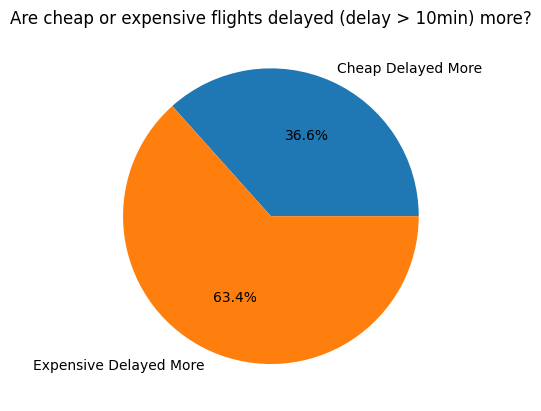
\includegraphics[scale=0.75]{images/DelayVsFare.png}

As is illustrated by this pie chart, the proportion of expensive flights that are delayed is much larger than the proportion of cheap flights being delayed. 

While this may seem counterintuitive due to the fact that airlines would likely prioritize higher paying customers, this disparity makes sense when considering the reason for more expensive flights. Cheaper flights are often early in the morning and the most expensive flights are at the most convenient times in the middle of the day. Airports run incredibly tight schedules, so when one flight gets delayed, this impacts the following flights. For this reason, it makes sense that cheap flights are delayed less as there are fewer opportunities for previous flights to cause delays.

In conclusion, there is correlation between the fare and the delay which gives us a basis to include it as a feature in our model. 

\section{Delay Prediction Model}
    \subsection{XGBoost}
    In the process of selecting the most suitable model for flight delay prediction, we considered several types of models. Linear regression was examined, but its assumption of linear relationships between predictor variables and the target variable made it less suitable for capturing the complex and non-linear nature of flight delays. Similarly, while decision trees are intuitive and capable of modeling non-linear relationships, the use of a single decision tree could lead to overfitting, prompting the exploration of ensemble methods to enhance predictive performance. Random Forest, an ensemble technique averaging multiple decision trees, offered improved robustness but lacked the fine-tuning capabilities and optimization features of our chosen model. Support Vector Regression (SVR) also stood as a formidable candidate due to its capacity to handle non-linear data. However, SVR's performance heavily relied on the appropriate selection of kernels and hyperparameter tuning, potentially requiring extensive computational resources which would not be compatible with the timeframe for this investigation.

    XGBoost emerged as the most compelling choice for our experiment. XGBoost's exceptional performance, scalability, and ability to handle tabular data containing numerical and categorical features rendered it well-suited for incorporating essential variables such as fare price, flight distance, and delay time in minutes. Its gradient boosting technique facilitated the creation of an ensemble of decision trees, effectively capturing complex non-linear relationships in the data. Moreover, XGBoost's inherent regularization mechanisms offered a means to mitigate overfitting, a crucial aspect in predicting flight delays given the intricacies and variability of airline operations.

    We ultimately decided to use XGBoost for its remarkable predictive performance, interpretability, scalability, and regularization capabilities, making it an ideal choice for accurately predicting flight delays.
    
    \subsection{Normalization}
    Working with the flight data had some unique challenges. Fare price, flight distance, and delay time (in minutes), have different scales. For example, the fare price could range from a few dollars to hundreds or even thousands, while the flight distance might vary from a few miles to thousands of miles. Delay time could range from zero (no delay) to potentially many hours. These different scales could lead to numerical instability during the training process. The different scales could also impact the adjustments made by the XGBoost gradient descent, as features with larger scale may cause the algorithm to take larger steps in that direction. It was also necessary to ensure that the features would be weighted equally by the model. Using normalized data, we were able to achieve a Root Mean Squared Error of .03 compared to 19.3.
    
    \subsubsection{Min-Max}

    To normalize the columns, a Min-Max normalization function was used where a data point would be assigned a value from 0 to 1, with 0 being the minimum value and 1 being the maximum value. This function would also be used for the model prediction function and inverse transformation of the prediction. 

    $$\textbf{Normalized Value} =\frac{Value-Value_{min}}{Value_{max}-Value_{min}} $$

    \subsection{Predictions}

    After training the model, could make predictions of a flight's airline delay time given the input of an airline, flight, and fare price. This prediction was output as a number in the range 0-1, so an inverse min-max function was used, taking into account the minimum and maximum values in the training dataset. In addition to a predicted delay time, the model would output a probability of a delay time greater than the predicted time. This information was used with an inverse cumulative distribution function used to calculate a distribution of possible delay times and respective probabilities for the given airline, flight, and fare price. 
    \begin{center}
    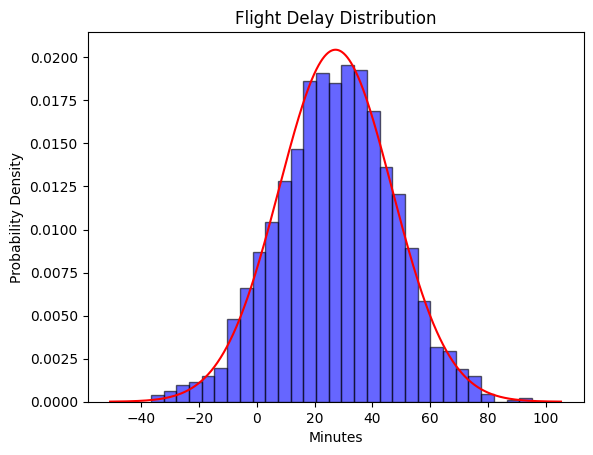
\includegraphics[scale=0.75]{images/output.png}
    \textbf{Figure 3}: Predicted Distribution of Airline Delays for an AA flight of 1700 miles with a fare price of \$300. Model output was 12.8 minutes with $P(Delay>Predicted \ Delay)$ of .77.
    \end{center}
    \section{Conclusion}
    In conclusion, our research on the US airline industry has provided valuable insights into the dynamics of flight fares and delays, contributing to a deeper understanding of this critical sector. Through a comprehensive analysis of the datasets provided, we investigated various factors surrounding the value of flight fares, their correlation with delays, and developed a predictive model for estimating delay times based on airline, distance, and fare price.

    Our investigation revealed that the average fare per mile varies significantly between airlines, with some carriers offering substantially better value compared to others. Additionally, we found a surprising correlation between fare prices and flight delays. Contrary to conventional belief, our results indicate that more expensive flights are more frequently delayed. This discrepancy can be attributed to factors like flight scheduling, airline operations, and the cascading effects of delays on subsequent flights.

    To provide a solution for anticipating delays and aiding travelers in their decision-making, we built a robust predictive model using XGBoost. The model allowed us to estimate the probability distribution of delay times for a given flight based on its airline, distance, and fare price. This information can be instrumental in helping passengers make informed decisions when purchasing tickets and planning for potential delays. We did not take into account weather delays, since it is difficult for an airline to control; rather, we only investigated whether price had a impact on delays that were an airline's fault.

    Overall, our research contributes to a better understanding of the interplay between fare prices and flight delays in the US airline industry. By providing insights into the factors affecting flight delays and offering a predictive model for delay estimation, this can help both the airlines and the passengers: by looking at this data, the airlines could make changes to help reduce delays, while the passengers could have a better 
    As our world continues to evolve, this comprehensive understanding of the airline industry remains crucial for sustaining global connectivity and economic prosperity. We hope our findings will drive further exploration and inform strategic decision-making in this ever-important sector of our economy.

    

\end{document}
